\documentclass[11pt,a4paper]{article}
\usepackage[margin=25mm]{geometry}

\usepackage[utf8]{inputenc}
\usepackage{amsmath,amssymb,amsthm,mathtools,booktabs,array,graphicx,microtype,tabularx}
\usepackage{xcolor,hyperref,xurl}
\hypersetup{colorlinks=true,linkcolor=blue,citecolor=blue,urlcolor=blue,
 pdftitle={Deletion, Arrows, Windows and Composition},
 pdfauthor={Alejandro Zarzuelo Urdiales}}
\setlength{\emergencystretch}{2em}
\newcommand{\R}{\mathbb R}
\newcommand{\Z}{\mathbb Z}
\newcommand{\Q}{\mathbb Q}
\newcommand{\code}[1]{\texttt{\nolinkurl{#1}}}
\newcommand{\lean}[1]{\texttt{#1}}
\newcommand{\repo}{https://github.com/alejandrozu/platonic-packing}
% Generated by scripts/patterns/paper_macros.py from docs/patterns/stats.json
\newcommand{\nRecords}{10,404}
\newcommand{\nFamilies}{140}
\newcommand{\nThreeD}{8,514}
\newcommand{\nFourD}{1,404}
\newcommand{\nFiveD}{279}
\newcommand{\nSixD}{207}
\newcommand{\nMonotone}{1,438}
\newcommand{\nAscend}{1,974}
\newcommand{\nDescend}{44}
\newcommand{\nHop}{1,168}
\newcommand{\nPerturb}{1,357}
\newcommand{\nLatcut}{142}
\newcommand{\nCompose}{63}
\newcommand{\nSymfresh}{134}
\newcommand{\nCommunity}{2,760}
\newcommand{\nLiterature}{112}
\newcommand{\nReinsert}{87}
\newcommand{\nFresh}{101}
\newcommand{\nPlateaus}{861}
\newcommand{\nPlateauRecords}{3,397}
\newcommand{\nComposites}{15}
\newcommand{\nNested}{63}
\newcommand{\nClosedForms}{1,624}
\newcommand{\nRational}{895}
\newcommand{\nSqrtTwo}{266}
\newcommand{\nSqrtThree}{185}
\newcommand{\nSqrtFive}{148}
\newcommand{\nFeat}{8,514}
\newcommand{\nLattice}{889}
\newcommand{\nLatticeOne}{685}
\newcommand{\nLatticeRational}{407}
\newcommand{\nSymTrivial}{7,738}
\newcommand{\nSymNontrivial}{776}
\newcommand{\nOneOrient}{1,241}
\newcommand{\nTwoOrient}{507}
\newcommand{\nInhFamilies}{86}
\newcommand{\nInhPairs}{20,124}
\newcommand{\nInhCons}{3,354}
\newcommand{\nInhConsFrozen}{601}
\newcommand{\nInhFrozen}{1,384}
\newcommand{\nInhPartial}{130}
\newcommand{\nRotRecords}{1,501}
\newcommand{\nRotPairs}{10,444}
\newcommand{\nRotRational}{3,303}
\newcommand{\nRotAllRational}{626}

\newcommand{\nCon}{2494}
\newcommand{\nConRattler}{649}
\newcommand{\pctConRattler}{26}
\newcommand{\nConIso}{107}
\newcommand{\meanCoord}{3.4}
\newcommand{\meanWall}{1.9}
\newcommand{\medExcess}{-39}
\newcommand{\liftWinPla}{2.77}
\newcommand{\pWinPla}{92}
\newcommand{\liftFroPla}{2.82}
\newcommand{\pFroPla}{94}
\newcommand{\liftIsoPla}{3.02}
\newcommand{\pIsoPla}{80}
\newcommand{\liftRatPla}{0.64}
\newcommand{\pRatPla}{17}
\newcommand{\liftRatWin}{0.03}
\newcommand{\nRatWin}{2}
\newcommand{\liftRatIns}{1.22}
\newcommand{\liftWinOne}{5.29}
\newcommand{\pWinOne}{77}
\newcommand{\liftSymWin}{4.92}
\newcommand{\liftWinRat}{3.60}
\newcommand{\liftCompRat}{7.25}
\newcommand{\liftClosedPla}{2.45}
\newcommand{\pClosedPla}{82}
\newcommand{\liftInsWin}{0.21}
\newcommand{\liftOptClosed}{5.41}
\newcommand{\liftSymRat}{0.00}
\newcommand{\nTrMatch}{19}
\newcommand{\nTrBeat}{0}
\newcommand{\nTrOne}{25}
\newcommand{\nTrFive}{181}
\newcommand{\nTrAll}{2475}
\newcommand{\nProven}{55}
\newcommand{\nNovel}{27}
\newcommand{\nPrism}{13}

\newcommand{\ndRecords}{1{,}890}
\newcommand{\ndFamilies}{54}
\newcommand{\ndFourRec}{1{,}404}
\newcommand{\ndFourOne}{17.5}
\newcommand{\ndFourSym}{20.0}
\newcommand{\ndFourPla}{21.1}
\newcommand{\ndFourRat}{12.6}
\newcommand{\ndFourLat}{264}
\newcommand{\ndFourFrz}{16.4}
\newcommand{\ndFiveRec}{279}
\newcommand{\ndFiveOne}{15.4}
\newcommand{\ndFiveSym}{22.6}
\newcommand{\ndFivePla}{17.6}
\newcommand{\ndFiveRat}{1.1}
\newcommand{\ndFiveLat}{41}
\newcommand{\ndFiveFrz}{16.7}
\newcommand{\ndSixRec}{207}
\newcommand{\ndSixOne}{15.9}
\newcommand{\ndSixSym}{24.6}
\newcommand{\ndSixPla}{22.7}
\newcommand{\ndSixRat}{1.4}
\newcommand{\ndSixLat}{12}
\newcommand{\ndSixFrz}{19.7}
\newcommand{\ndThreeOne}{14.6}
\newcommand{\ndThreeSym}{9.1}
\newcommand{\ndThreeFrz}{17.9}
\newcommand{\ndLiftSymOne}{3.8}
\newcommand{\ndLiftLatSym}{2.8}
\newcommand{\ndLiftPlaLat}{3.7}
\newcommand{\ndLiftPlaSym}{3.2}
\newcommand{\ndLiftCfSym}{3.4}
\newcommand{\ndSymCfive}{6.8}
\newcommand{\ndSymSxfive}{5.4}
\newcommand{\ndSymSxsix}{8.7}
\newcommand{\ndSymCeight}{32.9}
\newcommand{\ndSymHcfive}{36.6}
\newcommand{\ndSymHcsix}{36.2}
\newcommand{\ndIsoSixty}{96}
\newcommand{\ndSimpleFortyfive}{70}
\newcommand{\ndSimpleSeventytwo}{48}
\newcommand{\ndIsoFortyfive}{35}
\newcommand{\ndSimpleNinety}{29}

\newtheorem{theorem}{Theorem}
\newtheorem{proposition}[theorem]{Proposition}
\newtheorem{lemma}[theorem]{Lemma}
\theoremstyle{definition}
\newtheorem{definition}[theorem]{Definition}
\theoremstyle{remark}
\newtheorem{remark}[theorem]{Remark}

\title{Deletion, Arrows, Windows and Composition:\\a Classification of Structural Patterns in \nRecords{} Certified Polytope Packings}
\author{Alejandro Zarzuelo Urdiales}
\date{6 November 2026}

\begin{document}
\maketitle

\begin{abstract}
The Polyhedra-in-Polyhedra catalogue holds \nRecords{} certified packings of $n$ congruent convex polytopes in a scaled container, across \nFamilies{} problem families in dimensions 3--6. The records are far from structureless. We classify their recurring patterns into eleven classes: deletion and plateaus, subset relaxation (``arrows''), insertion and completion, composition and recursion, lattice windows, layers and orientation classes, symmetry, algebraic contact scales, extremal (provably optimal) configurations, contact structure, and transfer by inclusion. For each class we give a mechanism, prove it in Lean~4 with Mathlib where it is a theorem about packings, and measure how often it occurs across the catalogue. We then measure the relations between the classes. The formal implications are proved once for all bodies: lattice windows give plateaus, composition with a single piece gives the transfer bounds, and an extremal lower bound plus deletion proves a whole plateau optimal. Empirically, \pWinPla{}\% of lattice windows lie on plateaus. About a quarter of the records with $n\le30$ contain a rattler, but lattice windows almost never do (lift \liftRatWin{}). No transfer bound beats a record in the 25 Platonic families, and \nTrMatch{} records are exactly a transfer. A new box centre lemma for cube containers proves \nPrism{} prism-in-cube records optimal. Examples are triangular prisms of height 2 at side 2 for every $n$ from 2 to 6, which includes a new exact six-prism construction, and dodecagonal prisms at $2+\sqrt3$. Lemma F in dimension 5, with a new bound between Hosono's near-axis step and the elementary far region, proves side 2 optimal for 2 to 32 five-cubes in a five-cube. This brings the catalogue to \nProven{} records proven optimal in Lean. In dimensions 4--6, symmetric records are more than twice as common as in 3D, and the commonest rational relative rotations between orientation classes in 4D are the isoclinic $(60^\circ,60^\circ)$ of the 24-cell's triality and simple $45^\circ$ and $72^\circ$ turns. PingYou Ltd's arrows reproduce their square-antiprism bounds from catalogue records, and their submitted constructions for $N=2$--20 are now the records. Applied to other antiprism families, arrows improve 14 records, by up to $5\%$.
\end{abstract}

\section{Introduction}

A \emph{finite container packing} asks for the smallest scale $s(n)$ of a container $C$ holding $n$ congruent copies of a body $K$ with disjoint interiors. The Polyhedra-in-Polyhedra catalogue~\cite{archive} records, for \nFamilies{} pairs $(K,C)$ of Platonic, Archimedean and Catalan solids, prisms, antiprisms and regular polytopes in dimensions 4--6, the best certified packing found for each $n$ up to 100: \nThreeD{} records in 3D and \nFourD{}, \nFiveD{} and \nSixD{} in dimensions 4, 5 and 6. Every record carries an exact certificate of containment and pairwise separation. The packings come from soft-to-rigid continuation~\cite{nakajima2026,zarzueloMethods}, basin hopping, lattice cuts, composition, published constructions~\cite{berthold2026} and many community contributions, prominently those of PingYou Ltd, \code{konoha-ily2} and PolyPack.

Looking at the catalogue as data, the records are far from independent optima. They come in plateaus where $s(n)$ does not change. They are finite windows of lattice tilings, or compositions of smaller packings. They inherit large rigid blocks from neighbouring records. They show layered and symmetric arrangements, and their scales satisfy short algebraic equations. PingYou Ltd recently made two such observations explicit: an illustrated account of sixteen exact constructions and their number patterns~\cite{pingSixteen}, and ``arrows'' that recover smaller square-antiprism packings from a larger one~\cite{pingArrows}. This paper turns these observations into a classification with three layers:

\begin{enumerate}
\item \textbf{Mechanisms.} Each pattern class is a construction rule. Where the rule is a statement about packings, we prove it once in Lean~4~\cite{mathlib} for all bodies, containers and dimensions (Section~\ref{sec:formal}).
\item \textbf{Exact instances.} Catalogue records that realize a mechanism exactly are formalized at their exact scales, rather than the clearance-padded scales of the certified records.
\item \textbf{Prevalence.} Each class is measured over the whole catalogue by reproducible scripts (\code{scripts/patterns/}), and every number in this paper is generated from their output.
\end{enumerate}

Table~\ref{tab:taxonomy} summarizes the eleven classes. The remaining sections treat them in turn, measure the relations between them (Section~\ref{sec:relations}), classify the families (Section~\ref{sec:families}) and state the limits of the claims (Section~\ref{sec:limits}).

\begin{table}[t]
\centering\footnotesize
\begin{tabularx}{\textwidth}{>{\raggedright}p{2.6cm} >{\raggedright}X >{\raggedright}p{3.6cm} >{\raggedright\arraybackslash}p{3.4cm}}
\toprule
Class & Mechanism & Formal statement (Lean) & Prevalence \\
\midrule
P1 Deletion, plateaus & $m\le n$ pieces of an $n$-packing are an $m$-packing & \lean{Packing.restrict} & \nPlateaus{} plateaus, \nPlateauRecords{} records; \nMonotone{} records built by deletion \\
P2 Arrows & subset, then F (fixed orientations, LP), then P (free); insertions, kicks & \lean{Packing.restrict}, \lean{Packing.of\_separators} & PingYou's square-antiprism bounds reproduced; 14 antiprism records improved \\
P3 Insertion, completion & $(n-1)$-packing plus a piece in a hole & (constructive only) & \nAscend{} records built by insertion \\
P4 Composition & $s_{C}(Q,n)\,s_{Q}(P,m)$ bounds $s_C(P,nm)$ & \lean{Packing.compose}, \lean{Packing.pow} & \nComposites{} exact composites, \nNested{} nested records \\
P5 Lattice windows & Voronoi cells of distinct points & \lean{voronoi\_packing}, \lean{lattice\_window} & \nLattice{} windows (\nLatticeRational{} at rational scale) \\
P6 Layers, orientation classes & a few layers, few orientations & (descriptive) & \nOneOrient{} single-orientation records \\
P7 Symmetry & invariance under container symmetries & (descriptive) & \nSymNontrivial{} symmetric 3D records \\
P8 Algebraic scales & contact equations close the scale & (exact certificates) & \nClosedForms{} closed forms \\
P9 Extremal & lower bound meets construction & centre, width, box and volume lemmas; \lean{optimal\_plateau\_of\_*} & \nProven{} records proven optimal (Section~\ref{sec:extremal}) \\
P10 Contacts & contact graph, rattlers & (measured) & \nConRattler{} of \nCon{} records ($n\le30$) with a rattler \\
P11 Transfer & one piece of $K$ in $tK'$, or of $C'$ in $\lambda C$ & \lean{Packing.transfer\_piece}, \lean{transfer\_container} & \nTrMatch{} Platonic records equal a transfer, none beaten \\
\bottomrule
\end{tabularx}
\caption{The eleven pattern classes. Prevalence counts are over all \nRecords{} records, or over the \nFeat{} 3D records where a geometric feature is needed.}
\label{tab:taxonomy}
\end{table}

\section{Setting}

Let $E$ be a finite-dimensional real inner product space, $K,C\subseteq E$ and $s\ge 0$. A \emph{packing} of $n$ copies of $K$ in $s\,C$ is a family of affine isometries $g_1,\dots,g_n$ of $E$ with $g_i(K)\subseteq sC$ and $\operatorname{int} g_i(K)\cap \operatorname{int} g_j(K)=\emptyset$ for $i\neq j$. This is the structure \lean{Packing K C s n} of the Lean development (\code{lean-optimality/PackingOptimality/Basic.lean}). Reflections are allowed, so lower bounds proved for it hold for the catalogue's rotation-only packings. The catalogue measures $s$ as the ratio of container to piece edge (or linear size for Catalan solids). A record $r$ stores $s_{\mathrm{full}}(r)$, carrying a clearance of at least $10^{-7}$ between pieces and walls, and an exact certificate. The touching limit $s_{\mathrm{tight}}$ is what the patterns below are about.

\section{Deletion, plateaus and frozen subsets (P1)}\label{sec:deletion}

The simplest mechanism is deletion: any $m\le n$ pieces of an $n$-packing form an $m$-packing in the same container, so $s(m)\le s(n)$ (\lean{Packing.restrict}). The catalogue enforces this monotonicity: when a search finds $s(n+1)<s(n)$, the $(n+1)$-packing minus one piece replaces the $n$-record. \nMonotone{} records arose this way, and \nDescend{} more from an explicit deletion move.

\paragraph{Plateaus.} A plateau is a maximal run $n_0<\dots<n_1$ with $s(n_0)=\dots=s(n_1)$. The catalogue has \nPlateaus{} plateaus containing \nPlateauRecords{} records. The longest are $s=2$ for $2\le n\le 32$ five-cubes and $2\le n\le 24$ six-cubes (Hosono's centre lemma~\cite{hosono}). Others are $s=4$ for $39\le n\le 64$ cubes and $41\le n\le 64$ triangular prisms (grid tilings), $s=4$ for $37\le n\le 56$ truncated cubes (the Cartesian shell, Section~\ref{sec:windows}) and $s=5$ for $75\le n\le 93$ rhombic dodecahedra. A plateau ends at a \emph{window number}, the largest count a rigid construction holds at that scale. Most plateaus are deletions of a single lattice window or tiling.

\paragraph{Frozen subsets.} Deletion predicts a sharper relation between records. For records $k<N$ of one family, let $f(k,N)$ be the largest fraction of the $k$ pieces that can be matched one-to-one with pieces of the $N$-packing after a single container symmetry and translation, with matching centres and identical placed vertex sets (orientation included, up to the piece's own symmetry; tolerance $0.02$ edges; \code{scripts/patterns/inherit.py}). Then $f=1$ means record $k$ is literally $k$ pieces of record $N$, moved rigidly. Over \nInhPairs{} pairs with $N-k\le 6$ in \nInhFamilies{} families, \nInhFrozen{} pairs are frozen ($f=1$), \nInhConsFrozen{} of them consecutive ($N=k+1$). Figure~\ref{fig:inherit} shows the cube family. Frozen blocks appear exactly on the plateaus and on the $k^3$ grids. Between them, consecutive records share little rigidly: each was re-optimized after the deletion. Over all families, frozen pairs thin out with the gap: \nInhConsFrozen{} of the \nInhCons{} consecutive pairs are frozen, and fewer at each larger gap.

\begin{figure}[t]
\centering
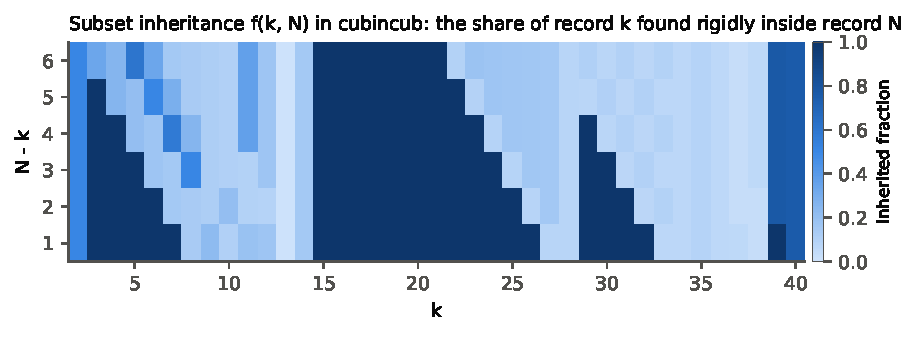
\includegraphics[width=\textwidth]{fig_inherit_cubincub.pdf}
\caption{Subset inheritance in cubes in a cube. Dark cells: record $k$ is a rigid subset of record $N$. The plateaus $s=2$ ($n\le 8$), $s=3$ ($15\le n\le 27$) and $s=4$ ($39\le n\le 64$) appear as solid blocks.}
\label{fig:inherit}
\end{figure}

\section{Arrows: subset relaxation and kicks (P2)}\label{sec:arrows}

PingYou Ltd observed that a larger packing contains good smaller ones that are \emph{not} rigid subsets: selecting six or eight square antiprisms of their 19-piece packing and relaxing them recovers their 6- and 8-piece bounds~\cite{pingArrows}. They specified the relaxation as two steps, with the unit bodies fixed throughout:

\begin{description}
\item[F] hold every orientation fixed and minimize the scale over the centres, re-selecting pair separation planes;
\item[P] minimize the scale with centres and rotations free, by a sequential linear program.
\end{description}

Arrows combine these with discrete moves: deletion (keep a subset), insertion (add a body at an affine guess or at the hub, the mean of the centres), and kicks (rotate one body about its own axis, or a group of bodies about an axis through their centroid, by $\pm 6^\circ$ to $\pm 16^\circ$), each followed by F then P.

\paragraph{F is an exact linear program.} With orientations $R_i$ fixed and one unit axis $u_{ij}$ chosen for each pair, write $h_i(u)=\max_{x\in K}\langle u,R_i x\rangle$. Every constraint is then linear in the centres $c_i$ and the scale $s$:
\begin{equation}\label{eq:F}
\langle N_f,c_i\rangle+h_i(N_f)\le \beta_f\,s\quad\text{(walls)},\qquad
\langle u_{ij},c_i\rangle+h_i(u_{ij})\le \langle u_{ij},c_j\rangle-h_j(-u_{ij})\quad\text{(pairs)},
\end{equation}
where $\{x:\langle N_f,x\rangle\le\beta_f\}$ are the container's facets. Any feasible point is a packing, since each pair is split by a plane: this is \lean{Packing.of\_separators}, proved for arbitrary bodies. Its optimum is therefore a certified packing for that choice of axes. F iterates by re-selecting each pair's best separating axis at the current point; the point stays feasible, so the scale never increases (\code{scripts/patterns/fp.py}).

\paragraph{Reproduction from catalogue records.} We ran arrows on the square-antiprism family $\mathrm{ap4}$ using only catalogue records as sources. The searches tried subsets of records with $N\le20$, chosen as caps along container directions, nearest clusters and random connected clusters. They then tried insertion and kicks from the improved packings (\code{scripts/patterns/arrows\_search.py}, \code{arrows\_kick.py}). Table~\ref{tab:arrows} lists the results. For $n=3$ and $5$--$9$ the arrows reach PingYou's bounds to every digit they announced, starting from different packings: their 19-piece packing was not in the catalogue. For $n=9$ their value is the closed form $1+2/(11-4\delta)$, $\delta=1+\sqrt2$. For $n=6$ the subset alone stops at $2.2500$. A single kick, a $16^\circ$ spin of one body about its own axis followed by F and P, reaches their value, which they had obtained by selecting six bodies of their 19-piece packing. For $n=10$ a single $6^\circ$ spin of the record reproduces their tighter certificate. For $n=11$--$14$ kicks improve the catalogue record but stay above PingYou's values. Those came from different constructions: relative square-face spins with receiver reflow, joint pair reinsertion, and ordered overlapping patches. The chain $6\to7\to8\to9$ follows their insertion arrows $N6\to N7$ and $N8\to N9$. When different starting points reach the same value, they have most likely reached the same rigid contact configuration by different arrows.

PingYou Ltd has since submitted their constructions for $N=2$--20 with exact certificates (pull request \#107). They pass the catalogue's verifier and exact certifier and are now the records. They improve $N=11$--20, with $N=15$--17 at exactly~3, and give exact endpoint certificates for $N=2$--10. For $N=3$ and $5$--$9$ their own witnesses replace our reproductions.

\paragraph{Arrows on other antiprisms.} The same subset arrows, started only from catalogue records of the pentagonal, hexagonal, octagonal and dodecagonal antiprism families, improve 14 records (all certified). The largest gains are hexagonal antiprisms at $n=6$, from $2.2466$ to $2.1518$, and octagonal antiprisms at $n=9$ and $10$, from $2.7464$ to $2.6249$ and from $2.8515$ to $2.7118$. Each came from a subset of a record with 11 to 13 pieces. Two of the new pentagonal-antiprism values match short closed forms, $(11-\sqrt5)/4$ at $n=6$ and $(7-\sqrt5)/2$ at $n=8$. These are conjectures until the contact systems are solved.

\begin{table}[t]
\centering\small
\resizebox{\textwidth}{!}{\begin{tabular}{rllll}
\toprule
$n$ & catalogue record & arrow from catalogue records & scale reached & PingYou Ltd~\cite{pingArrows} \\
\midrule
3 & 1.973017314 & subset $\{4,6,12\}$ of $N=15$, F, P & 1.9726490831 & 1.972649083082090 \\
5 & 2.209265853 & subset of $N=9$, F, P & 2.1785815015 & 2.178581501510501 \\
6 & 2.292893610 & subset of $N=9$, F, P; spin $16^\circ$, F, P & 2.2459217996 & 2.245921799598007 \\
7 & 2.373563494 & insert into $n=6$ (affine guess); four spins, F, P after each & 2.3629758095 & 2.362975810 \\
8 & 2.402020630 & insert into $n=7$; four spins & 2.3849425743 & 2.384942574336931 \\
9 & 2.542195713 & hub insertion into $n=8$, F, P & 2.4890416764 & $1+2/(11-4\delta)$ \\
10 & 2.590076603 & spin $6^\circ$ of the record, F, P & 2.5900761895 & 2.590076189471171 \\
11 & 2.743255848 & kicks of the record, F, P after each & 2.7406579330 & 2.652646434968480 \\
12 & 2.807780046 & kicks of the record & 2.8008665059 & 2.764993777408391 \\
13 & 2.907150931 & kicks of the record & 2.8905573692 & 2.842219125707920 \\
14 & 2.970067187 & kicks of the record & 2.9543988095 & 2.945858498562152 \\
\bottomrule
\end{tabular}}
\caption{Arrows on square antiprisms in a square antiprism, from catalogue records only. ``Scale reached'' is the touching limit after F and P. The certified records add $10^{-7}$ clearance. The last column is PingYou's value. Their submitted constructions for $N=2$--20 are now the catalogue records.}
\label{tab:arrows}
\end{table}

\begin{figure}[t]
\centering
\includegraphics[width=0.9\textwidth]{fig_arrow.pdf}
\caption{An arrow: three square antiprisms of the 15-piece record, then F and P, reach $S_3=1.9726490831$.}
\label{fig:arrow}
\end{figure}

\section{Insertion and completion (P3)}

The converse of deletion adds a piece to an $(n-1)$-packing, in its largest hole, and re-sharpens (\nAscend{} records). A rigid version is \emph{completion}: a construction with empty corners or gaps receives additional pieces at the same or slightly larger scale. PingYou's 61 truncated cubes~\cite{pingSixteen} complete the 56-piece Cartesian shell (Section~\ref{sec:windows}) with five corner pieces. The 40 wall and contact inequalities of their contact system sum to $5(2+\sqrt2)(S-1)\ge 60$, so $S\ge 13-6\sqrt2$, and the construction attains it. That bound holds for the declared contact system, not for all packings. Insertion arrows (PingYou's $N6\to N7$ and $N8\to N9$, the latter with a hub body of orientation $\operatorname{diag}(1,-1,-1)$) are completion followed by F and P.

\section{Composition and recursion (P4)}\label{sec:compose}

Scales are ratios, so they multiply.

\begin{theorem}[\lean{Packing.compose}]\label{thm:compose}
If $n$ copies of $Q$ pack in $s\,C$ and $m$ copies of $P$ pack in $t\,Q$ with $t\ne 0$, then $nm$ copies of $P$ pack in $(st)\,C$. In particular, for $K=P=Q=C$, $s(nm)\le s(n)\,s(m)$ (\lean{Packing.selfCompose}) and $s(n^k)\le s(n)^k$ (\lean{Packing.pow}).
\end{theorem}

\begin{proof}[Proof sketch]
Conjugating $g$ by the dilation $x\mapsto tx$ gives $\hat g=x\mapsto t\,g(0)+\vec g(x)$ with $\hat g(tA)=t\,g(A)$. The pieces $\hat g_i(h_j(P))\subseteq t\,g_i(Q)\subseteq (st)\,C$ are disjoint within one $g_i$ because $\hat g_i$ is an isometry. Across $i\ne i'$ they are disjoint because the interiors of $t\,g_i(Q)$ and $t\,g_{i'}(Q)$ are.
\end{proof}

Nested composition is how \nNested{} records were built (\code{scripts/compose3d.py}, \code{compose\_nd.py}; the whole-body inclusion idea is PingYou's contribution~\cite{ping79}). In the self-similar families, \nComposites{} records equal a product $s(n)s(m)$ exactly. They include the cube and prism tilings ($64=8\cdot 8$ at scale 4) and the rhombic-dodecahedron record $36=6\cdot6$ at 4. The cleanest is the triakis tetrahedron, where PingYou recognized the 16- and 64-piece records as the 4-piece packing squared and cubed~\cite{pingSixteen}.

\begin{theorem}[\lean{triakis\_recursion}]\label{thm:triakis}
For every $k\ge0$, $4^k$ triakis tetrahedra pack in a triakis tetrahedron of scale $(5/3)^k$.
\end{theorem}

\begin{proof}
Write the catalogue's triakis tetrahedron as $\{x:\langle m,x\rangle\le 9\sqrt2/4\}$ over its twelve integer face normals $m$ (of type $(1,3,1)$). Place piece $i$ at $R_iK+(\sqrt2/2)\sigma_i$ with $\sigma_i\in\{(-1,1,1),(-1,-1,-1),(1,1,-1),(1,-1,1)\}$ and rotations $R_i$ with entries $\pm\frac13,\pm\frac23$. Containment in $\frac53K$ is a linear consequence of the face inequalities. The six pairs touch along the planes $x_a\pm x_b=0$. This gives the 4-piece packing at $5/3$ (\lean{Triakis.ktt4}); Theorem~\ref{thm:compose} gives the powers.
\end{proof}

\section{Lattice windows and tilings (P5)}\label{sec:windows}

\begin{theorem}[\lean{voronoi\_disjoint}, \lean{voronoi\_packing}]
If $A$ lies in the Voronoi half-space of $p$ against $q$ and $B$ in that of $q$ against $p$ ($p\ne q$), then $A$ and $B$ have disjoint interiors. Hence copies $g_i(K)$ lying in the Voronoi cells of distinct centres $c_i$, inside $sC$, form a packing. For a lattice $\Lambda$ whose Voronoi cell contains $K$, any finite set of translates of $K$ by points of $\Lambda$ that fit in $sC$ is a packing (\lean{lattice\_window}).
\end{theorem}

The proof separates $A$ and $B$ by the bisector $\langle q-p,x\rangle=(\|q\|^2-\|p\|^2)/2$. The theorem turns every lattice window into a finite containment check, and it covers multi-orientation windows whose pieces lie in the Voronoi cells of their centres. We formalize two families completely (\code{Windows.lean}):

\begin{itemize}
\item \textbf{Rhombic dodecahedra.} $R=\{|x_i|+|x_j|\le1\}$ is the Voronoi cell of $D_3$, the FCC lattice. For $x\in R$ and $v\in D_3$ one has $2\langle x,v\rangle\le\|v\|^2$. The support function of $R$ is $\max(\|v\|_\infty,\|v\|_1/2)$, and both terms are at most $\|v\|^2/2$ on $D_3\setminus0$ (\lean{rd\_voronoi}). Every window $\{w\in D_3:|2w_i+e_i|+|2w_j+e_j|\le M\}$ packs in $(M/2+1)R$ (\lean{rdo\_window}). The catalogue's records of 19, 44 and 93 pieces at scales 3, 4 and 5 are such windows: the FCC shell $1+12+6$ and the palindromic window $2+8+12+12+8+2$ of PingYou~\cite{pingSixteen}, and the 93-piece record. They are proved at the exact scales, and by deletion every smaller count at the same scale.
\item \textbf{Truncated cubes.} The unit-edge truncated cube $T$ lies in the Voronoi cell $[-a,a]^3$ of $2a\Z^3$, with $a=(1+\sqrt2)/2$. The $4\times4\times4$ grid minus its eight corners packs 56 copies in $4T$ (\lean{tcu56}): PingYou's Cartesian shell $56=4^3-2^3$, the end of the plateau $37\le n\le56$.
\end{itemize}

Over the 3D catalogue, \nLattice{} records are lattice windows: every orientation class with at least four pieces sits on a lattice, with at most four classes. \nLatticeOne{} of them have a single orientation, and \nLatticeRational{} sit at a rational scale. Figure~\ref{fig:windows} shows how the window numbers terminate the plateaus. Two-orientation windows include PingYou's truncated-tetrahedron windows: 35 = 19 + 16 at $11/3$ and 71 = 40 + 31 at $13/3$, the two counts being coefficients of $(1+x+x^2)^4$ and $(1+x+x^2+x^3)^4$~\cite{pingSixteen}.

\begin{figure}[t]
\centering
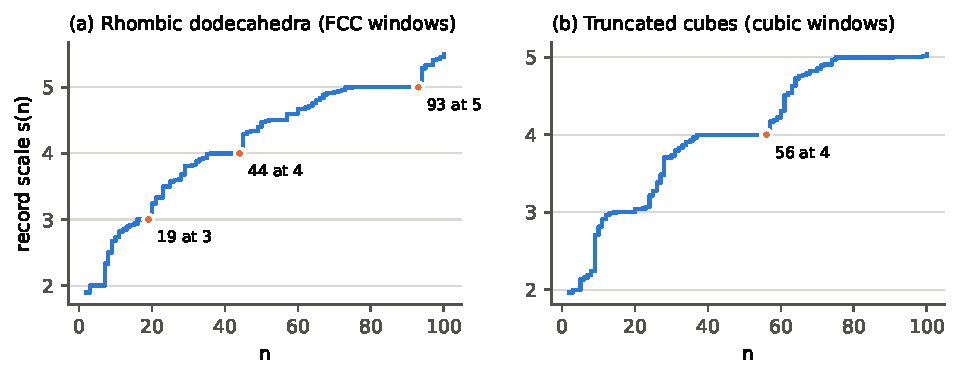
\includegraphics[width=\textwidth]{fig_windows.pdf}
\caption{Record scales against $n$. Plateaus end at lattice window numbers: 19, 44 and 93 FCC windows of rhombic dodecahedra at scales 3, 4 and 5, and the 56-piece Cartesian shell of truncated cubes at scale 4 (all proved in Lean at the exact scales).}
\label{fig:windows}
\end{figure}

\section{Layers and orientation classes (P6)}

Many records are stacks of a few layers, with only a few orientations of the pieces up to the piece's own symmetry. Over the 3D catalogue, \nOneOrient{} records use a single orientation and \nTwoOrient{} use exactly two (Figure~\ref{fig:sym}b). Layer inventories along a container direction give the number patterns PingYou highlights. Examples are $29=9+11+9$ and $30=9+12+9$ cubes in a dodecahedron, whose shared row phase forces the scales $5/\varphi^2$ and $23-13\varphi$. Others are $32=8+6\cdot4$ cubes in an icosahedron at $8/\varphi^2$, $44=6+6+32$ octagonal prisms at $4+2\sqrt2$, and $20=2\times2\times5$ dodecagonal prisms at $15/2$~\cite{pingSixteen}. The extraction is in \code{scripts/patterns/features.py}. It groups centres into layers along each container facet normal, and pieces into orientation classes when $R_i^{-1}R_j$ is a proper symmetry of the piece.

\paragraph{Relative orientations.} Between two orientation classes $a,b$, the relative rotation $R_a^{-1}R_b$ is defined modulo the piece's proper symmetries. We take the smallest angle over that coset (\code{scripts/patterns/rotations.py}). Over the \nRotRecords{} 3D records with two to eight classes, \nRotPairs{} class pairs give \nRotRational{} rational angles, that is, $p/q$ of a full turn with $q\le24$. In \nRotAllRational{} records every relative rotation is rational. The rational angles are the pieces' own symmetry angles: $90^\circ$ (1/4 turn), $60^\circ$, $30^\circ$, $36^\circ$, $45^\circ$, $18^\circ$, $15^\circ$ and $22.5^\circ$, in decreasing frequency. The remaining angles are not random either. They cluster at a few algebraic values, each tied to a family (Table~\ref{tab:angles}). Those values compose a symmetry rotation of the piece with a symmetry rotation of the container. Examples are $\arccos(-1/4)$ and $\arccos((\sqrt3-2)/4)$ for triangular prisms laid along different cube axes, and $\arccos(7/9)$ for octahedra in a cube.

\begin{table}[t]
\centering\small
\resizebox{\textwidth}{!}{\begin{tabular}{rlrl}
\toprule
angle & $\cos\theta$ & class pairs & main families \\
\midrule
$93.841^\circ$ & $(\sqrt3-2)/4$ & 662 & triangular prisms (heights 1, 1.5, 2, 3) in a cube \\
$37.399^\circ$ & $(4\sqrt5-1)/10$ & 167 & dodecahedra in a dodecahedron, icosahedron, octahedron \\
$104.478^\circ$ & $-1/4$ & 112 & triangular prisms in a cube \\
$15.631^\circ$ & -- & 98 & triangular and hexagonal prisms in a cube (twist about the prism axis) \\
$95.480^\circ$ & $(\sqrt5-3)/8$ & 48 & pentagonal prisms in a cube \\
$62.799^\circ$ & $(2\sqrt2-1)/4$ & 46 & cubes in a cube \\
$38.942^\circ$ & $7/9$ & 36 & octahedra in a cube \\
\bottomrule
\end{tabular}}
\caption{Recurring non-rational relative orientations between orientation classes. The cosines are matched to $3\times10^{-6}$ and are conjectural; one cluster is not identified at this precision.}
\label{tab:angles}
\end{table}

\section{Symmetry (P7)}

The configuration symmetry group of a record is the set of container symmetries, reflections included, that map the set of placed pieces onto itself. It is computed exactly on placed vertex sets at tolerance $10^{-4}$ edges. Of the \nFeat{} 3D records, \nSymTrivial{} are asymmetric and \nSymNontrivial{} have a nontrivial group (Figure~\ref{fig:sym}a). The fully symmetric records (orders 24, 48 and 120) are all windows or shells. Symmetric seeding (\nSymfresh{} records) was one of the search moves, but most symmetric records come from lattice cuts and contributed constructions. Relaxation from a symmetric start rarely keeps the symmetry.

\begin{figure}[t]
\centering
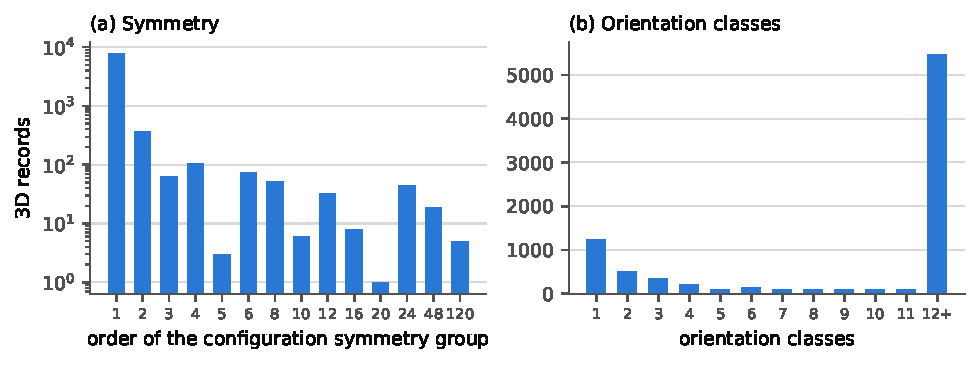
\includegraphics[width=\textwidth]{fig_sym_orient.pdf}
\caption{(a) Orders of configuration symmetry groups of the \nFeat{} 3D records (log scale). (b) Number of orientation classes.}
\label{fig:sym}
\end{figure}

\section{Rotations, symmetry and subsets in dimensions 4--6}\label{sec:nd}

The measures of Sections~\ref{sec:deletion}--\ref{sec:extremal} apply unchanged to the \ndRecords{} records of the \ndFamilies{} families of regular polytopes in dimensions 4--6 (\code{scripts/patterns/features\_nd.py}). The symmetry groups are computed from the vertex sets, by backtracking over vertex images with the Gram matrix of a basis of neighbouring vertices, and checked against their orders (120 for the 5-cell, 384 for the tesseract and 16-cell, 1152 for the 24-cell, 14\,400 for the 600- and 120-cells, 720, 3840 and 46\,080 for the simplex, cube and cross-polytope in 5D and 6D, and 5040 for the 6-simplex). A relative rotation $R_a^{-1}R_b$ is reduced modulo the piece's proper symmetries to the representative closest to the identity, and described by its rotation angles, one per invariant plane. It is \emph{simple} if one angle is nonzero and \emph{isoclinic} if all are equal.

\begin{table}[t]
\centering\small
\begin{tabular}{lrrrr}
\toprule
 & 3D & 4D & 5D & 6D \\
\midrule
records & 8514 & \ndFourRec & \ndFiveRec & \ndSixRec \\
one orientation class (\%) & \ndThreeOne & \ndFourOne & \ndFiveOne & \ndSixOne \\
nontrivial configuration symmetry (\%) & \ndThreeSym & \ndFourSym & \ndFiveSym & \ndSixSym \\
on a plateau (\%) & & \ndFourPla & \ndFivePla & \ndSixPla \\
consecutive records frozen (\%) & \ndThreeFrz & \ndFourFrz & \ndFiveFrz & \ndSixFrz \\
rational relative rotations (\%) & & \ndFourRat & \ndFiveRat & \ndSixRat \\
lattice windows & 889 & \ndFourLat & \ndFiveLat & \ndSixLat \\
\bottomrule
\end{tabular}
\caption{The pattern measures by dimension. The 3D plateau and rotation figures use other denominators (Section~\ref{sec:deletion} and P6) and are left out.}
\label{tab:nd}
\end{table}

Table~\ref{tab:nd} compares the dimensions. Three observations stand out.
\begin{itemize}
\item \textbf{Symmetry depends on the container.} Records in a simplex are almost never symmetric (5-cell \ndSymCfive\%, 5-simplex \ndSymSxfive\%, 6-simplex \ndSymSxsix\%), and few have a single orientation class (3.8\%, 0\% and 1.4\%). Records in a cube are the most symmetric (tesseract \ndSymCeight\%, 5-cube \ndSymHcfive\%, 6-cube \ndSymHcsix\%). Some records carry the container's whole group: 25 24-cells in a 24-cell (order 1152), and 10 and 12 cross-polytopes in the 5- and 6-cross-polytope (orders 3840 and 46\,080), with one piece towards each vertex of the container and, in the 24-cell, one more at the centre.
\item \textbf{Relative rotations in 4D are isoclinic or simple.} The commonest rational relative rotations are the isoclinic $(60^\circ,60^\circ)$ (\ndIsoSixty{} class pairs), the simple $45^\circ$ (\ndSimpleFortyfive), the simple $72^\circ$ (\ndSimpleSeventytwo), the isoclinic $(45^\circ,45^\circ)$ (\ndIsoFortyfive) and the simple $90^\circ$ (\ndSimpleNinety). The $60^\circ$ isoclinic rotations are left multiplications by unit quaternions of order 3 or 6, which permute the three 16-cells inscribed in a 24-cell. Accordingly, 24 16-cells in a 24-cell (scale $\sqrt2$, symmetry 1152) and 24 16-cells in a 600-cell come in three classes of eight. The $72^\circ$ rotations come from the 600- and 120-cells. In 5D and 6D almost no relative rotation is rational.
\item \textbf{The relations of Section~\ref{sec:relations} persist.} Over the 4D--6D records the lifts are \ndLiftSymOne{} (symmetric given one orientation class), \ndLiftLatSym{} (lattice given symmetric), \ndLiftPlaLat{} (plateau given lattice), \ndLiftPlaSym{} (plateau given symmetric) and \ndLiftCfSym{} (closed form given symmetric). About one consecutive pair in six is a frozen subset in every dimension. The most frozen pairs are in the cube families and the 24-cell, whose records are grids and shells.
\end{itemize}

\section{Algebraic scales (P8)}

A rigid record is a solution of its contact system: equalities between support functions of touching pieces and walls. Its scale is then algebraic. \nClosedForms{} records carry a conjectured closed form matched to $10^{-11}$: \nRational{} rational, \nSqrtTwo{} in $\Q(\sqrt2)$, \nSqrtThree{} in $\Q(\sqrt3)$ and \nSqrtFive{} in $\Q(\sqrt5)$, the rest in nested or biquadratic fields. The field reflects the geometry of the contacts. Golden scales come from dodecahedral and icosahedral walls, silver ratios $\delta=1+\sqrt2$ from square antiprisms (PingYou's $S_2\le(5-\delta)/\sqrt\delta$, $S_9\le1+2/(11-4\delta)$, $S_{20}\le3+1/(\delta+2)$~\cite{pingArrows}), and $\sqrt3$ from hexagonal and dodecagonal prisms. A closed form is an exact statement only once the contact system is solved and certified; PingYou's ``six-equation'', ``77-equation'' and ``115-equation'' contact constructions are such certificates~\cite{pingArrows}.

\section{Extremal patterns: proven optimality (P9)}\label{sec:extremal}

At the extreme of the classification are records whose scale is matched by a lower bound. \nProven{} catalogue records are proven optimal in Lean, \nNovel{} of them for the first time. Four mechanisms occur.
\begin{itemize}
\item \textbf{Volume tilings.} $k^d$ cubes and $k^3$ triangular prisms at scale $k$ (\code{Cubes.lean}, \code{Prisms.lean}).
\item \textbf{Centre lemmas for $n=2$ and plateaus.} If every piece at scale below $s$ contains the container's centre, then $s(2)\ge s$. Proven instances include the cube centre lemma in dimensions 3, 4 and 5 (plateaus $s=2$ for $2\le n\le 8$ cubes, $2\le n\le 16$ tesseracts and $2\le n\le 32$ 5-cubes), and the octahedron lemma (2 octahedra in a cube, $\sqrt2$). In dimension 5 the band between Hosono's near-axis step and the elementary far bound is new. There each zero-sum column vector is paired with its own column, turned in the plane of $e_1$ and the first column to a fixed direction at about $56^\circ$, and a sphere bound $\sum_i(s_i^3+\lambda s_i)\le U(\lambda)$ closes the inequality. Lean checks its 1174 interval cases.
\item \textbf{Elementary bounds.} The facet-width and two-ball lemmas prove optimality of 2 tetrahedra in a cube, octahedron, dodecahedron and icosahedron; 2 five-simplices in a 5-cube (the Paley construction); 2 five-cells in a 24-cell; and 2 16-, 24-, 120- and 600-cells in a tesseract or 16-cell.
\item \textbf{Widths and boxes in a cube.} In a cube a placed piece can be translated independently along each axis, so its admissible translations form a box. Two consequences follow. A piece has width at most $s$ along each axis (\lean{width\_le}). For every facet $(\beta,h)$ and any points $v_i$ of the piece, the centre of the cube satisfies $\langle\beta,y\rangle\le \tfrac s2\sum_i|b_i|+\sum_i b_i(Lv_i)_i$ in piece coordinates, with $b=L\beta$. For the best $v_i$ this is sharp (\lean{centre\_of\_box}). If the right side is below $h$ for every facet, the centre lies inside every placed piece.
\end{itemize}

The last mechanism proves \nPrism{} prism-in-cube records optimal (\code{PrismCube.lean}, \code{TriPrismCube.lean}, \code{PolyPrism.lean}):
\begin{itemize}
\item Triangular prisms of height 2: side 2 for every $n$ from 2 to 6. Widths force every coordinate of the axis below $13/19$. The caps hold because $\|a\|_1\le\sqrt3<2$. Each side reduces to $\sum_i|b_i|(1-|a_i|)\le\sqrt3/2$ for unit $b\perp a$: add a multiple of $\sum_ia_ib_i=0$, apply Cauchy--Schwarz, and use a sign argument, with $\sum_i|a_i|\ge 115/71$. Six prisms fit at side exactly 2. In each half of the cube, three prisms form a strip of alternating triangles, along different axes in the two halves. This improves the catalogue's $2.0000000034$ for $n=6$.
\item Triangular prisms of height $3/2$: side $3/2$ for $n=2,3$, because one prism already needs it. Some coordinate has $a_i^2\ge1/3$, and the triangle's six vertex differences at $60^\circ$ steps give width at least $\tfrac32|a_i|+\tfrac{\sqrt3}2\sqrt{1-a_i^2}\ge\tfrac32$. Three prisms fit at exactly $3/2$: their bases form a pinwheel in the square of side $3/2$, each base touching the other two.
\item Dodecagonal prisms: side $2+\sqrt3$ for height 1 ($n=2,3$) and height $3/2$ ($n=2$); side 4 for height 2 ($n=2$). Octagonal prisms of height 1: side $1+\sqrt2$ ($n=2$). Hexagonal prisms of height 1: side 2 ($n=2$). The thresholds are exact: for height 1, widths force $|a_i|>4\rho/(4\rho^2+1)$, which is $1/2$ for the dodecagon and $1/\sqrt2$ for the octagon. For the hexagon the side condition is $\|b\|_1\le\sqrt3=2\rho$.
\end{itemize}
Each of these results has the form of a general relation (Section~\ref{sec:relations}): an extremal lower bound plus deletion proves a whole plateau (\lean{optimal\_plateau\_of\_common\_point}, \lean{optimal\_plateau\_of\_one\_piece}). The numerical survey (\code{scripts/optimality/}) shows that the centre argument, or the one-piece bound, is also exact for 4-, 5- and 12-gonal antiprisms and for several further prisms in a cube. These are the next candidates. The results are recorded in \code{docs/OPTIMALITY.md}, and they explain where several plateaus start: a plateau begins where the lower bound is tight.

\section{Contact graphs and rattlers (P10)}\label{sec:contacts}

The contact graph of a record joins two pieces when their best separating plane has margin below $10^{-5}$, and a piece to a wall when a container facet is that close (\code{scripts/patterns/contacts.py}; the certified records carry $10^{-7}$ clearance, so touching pairs sit near $10^{-7}$). A \emph{rattler} is a piece that touches neither another piece nor a wall. Over the \nCon{} 3D records with $n\le30$, pieces have \meanCoord{} piece contacts and \meanWall{} wall contacts on average, and \nConRattler{} records (\pctConRattler\%) contain a rattler. A rattler can be deleted without changing the scale, so its record is an $(n-1)$-configuration at scale $s(n)$. The relations are sharp. Rattlers are rare on plateaus (lift \liftRatPla{}), almost absent from lattice windows (lift \liftRatWin{}, \nRatWin{} records) and absent from symmetric records. They lean towards records built by insertion (lift \liftRatIns{}). The \nConIso{} records whose contact count reaches the $6n+1$ degrees of freedom of the scale problem are mostly windows and plateau records (\pIsoPla\% on a plateau, lift \liftIsoPla{}). Plateaus are rigid windows minus pieces, not loose packings, and a rattler marks an irregular record whose remaining pieces set the scale.

\section{Transfer by inclusion (P11)}\label{sec:transfer}

Composition with a single inner piece links different families. If one copy of $K$ fits in $tK'$, every packing of $n$ copies of $K'$ in $sC$ gives $n$ copies of $K$ in $(st)C$ (\lean{Packing.transfer\_piece}). If one copy of $C'$ fits in $\lambda C$, every packing of $K$ in $sC'$ gives one in $(\lambda s)C$ (\lean{Packing.transfer\_container}). Both are Theorem~\ref{thm:compose} with $m=1$ or $n=1$. For the 25 Platonic families we computed the twenty one-piece scales $s_1(K\text{ in }K')$ numerically (\code{scripts/patterns/transfer.py}). Examples are $s_1(\text{tet in cube})=1/\sqrt2$, $s_1(\text{cube in octahedron})=1+1/\sqrt2$ and $s_1(\text{cube in dodecahedron})=1/\varphi$. We then compared every record with the best transfer bound from a neighbouring family. No transfer bound beats a record. \nTrMatch{} records are exactly a transfer: cubes in a dodecahedron for $n=6$--8, 25--27 and 61--64 are the cube grids in the dodecahedron's inscribed cube ($1/\varphi$ times the cube records); 2 and 3 tetrahedra in a dodecahedron and 8 cubes in an octahedron likewise sit in an inscribed cube; and icosahedra in a cube ($n=8$, from $s_1(\text{ico in cube})=\varphi$) and in an octahedron ($n=10$ and 86--88) inherit cube and octahedron packings piece by piece. Of the \nTrAll{} record comparisons, \nTrOne{} are within $1\%$ of the transfer bound and \nTrFive{} within $5\%$. Transfer is therefore a consistency check on the catalogue, and a cheap source of starting points.

\section{Relations between the classes}\label{sec:relations}

A record usually belongs to several classes, and the classes are not independent. Figure~\ref{fig:relations} shows both kinds of relation.

\paragraph{Formal implications.} These are theorems in Lean, for arbitrary bodies and containers (\code{Relations.lean}, \code{Patterns.lean}, \code{Basic.lean}):
\begin{itemize}
\item a lattice window of $N$ pieces gives every $n\le N$ at the same scale, so windows end plateaus (\lean{lattice\_windows});
\item composition with one piece is transfer (\lean{transfer\_piece}, \lean{transfer\_container});
\item deletion and separator certificates make the arrows' F step sound (\lean{restrict}, \lean{of\_separators});
\item an extremal lower bound (centre, width, box or volume lemma) together with deletion proves every record of a plateau optimal (\lean{optimal\_plateau\_of\_common\_point}, \lean{optimal\_plateau\_of\_one\_piece}).
\end{itemize}

\paragraph{Empirical associations.} For classes $A$ and $B$, the lift $P(B\mid A)/P(B)$ over the 3D records measures how much more often $B$ occurs among records in $A$ (\code{scripts/patterns/relations.py}). The strongest relations are:
\begin{itemize}
\item \textbf{the rigid cluster.} Lattice windows, a single orientation class, symmetry, composites and rational scales attract one another (lifts 3.6 to 7.2). \pWinOne\% of windows have one orientation class (lift \liftWinOne{}), symmetric records are windows \liftSymWin{} times as often as average, and composites have rational scales \liftCompRat{} times as often.
\item \textbf{rigidity gives plateaus.} \pWinPla\% of windows and \pFroPla\% of frozen subsets lie on plateaus (lifts \liftWinPla{} and \liftFroPla{}), as do \pClosedPla\% of the records with a closed form.
\item \textbf{insertion and rattlers avoid the rigid cluster.} Records built by insertion are windows a fifth as often as average (lift \liftInsWin{}), and rattlers almost never occur in windows or symmetric records.
\item \textbf{proven optimality} goes with closed forms (lift \liftOptClosed{}). Every proof so far is for an exact, algebraic construction.
\end{itemize}
The associations are measurements on this catalogue, not theorems. They do show where to search. Irregular records built by insertion, especially those with a rattler, are where arrows and re-optimization find gains. The rigid cluster is where exact constructions and proofs are found.

\begin{figure}[t]
\centering
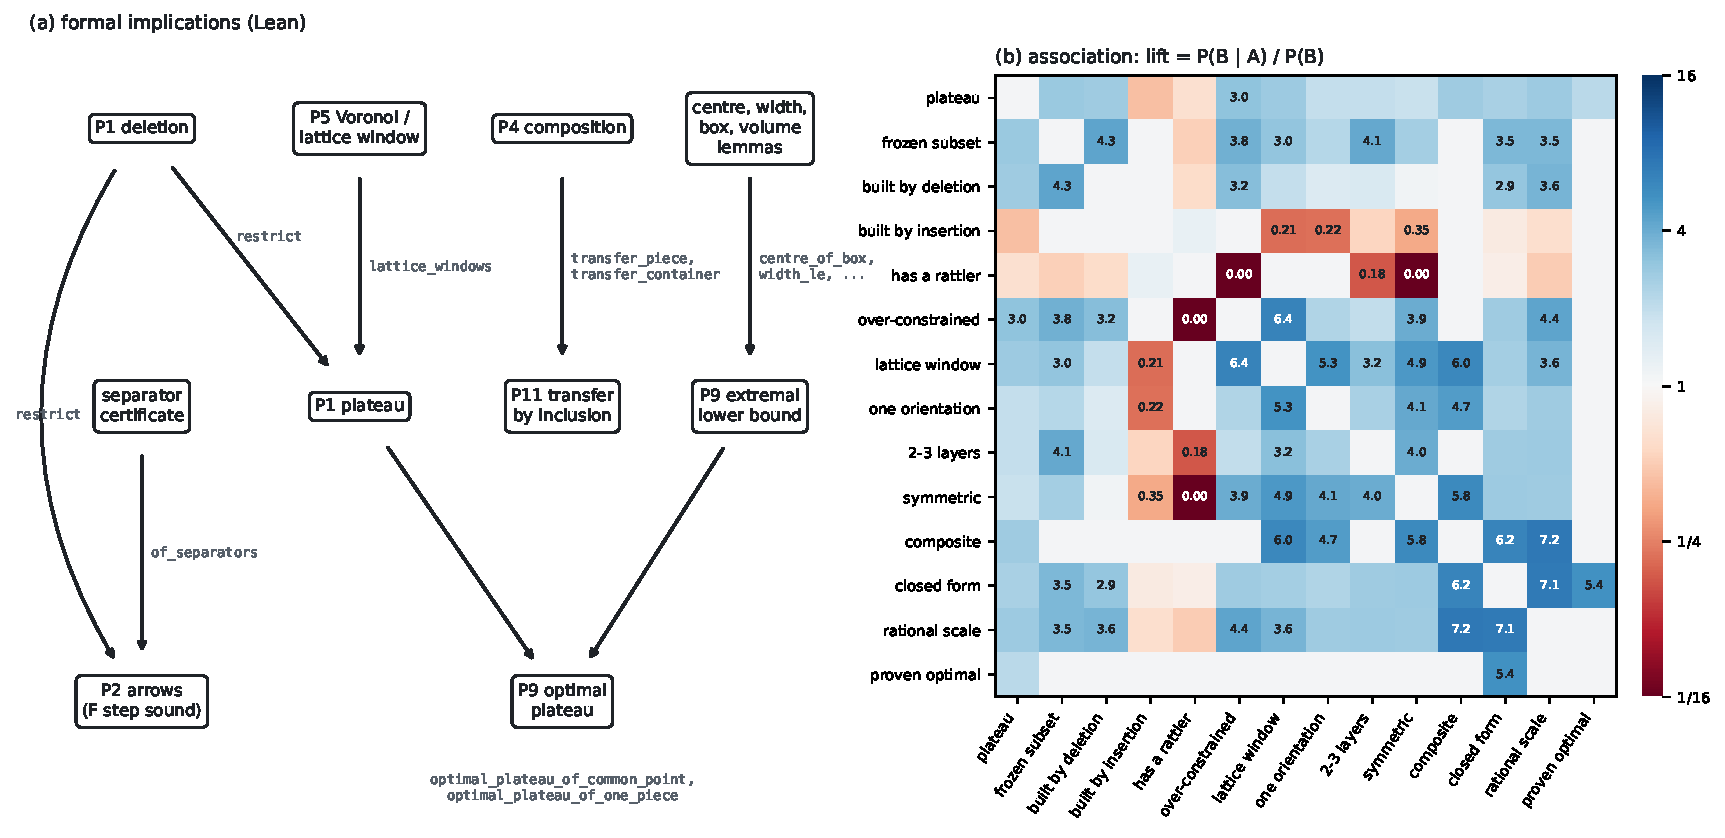
\includegraphics[width=\textwidth]{fig_relations.pdf}
\caption{Relations between the pattern classes. (a) Formal implications, with the Lean theorem on each arrow. (b) Empirical lift $P(B\mid A)/P(B)$ over the 3D records (contact features for $n\le30$). Blue: $B$ more frequent among records in $A$. Red: less frequent. White: independent. Grey: fewer than 20 joint records. Deletion and insertion, the last lineage move, are exclusive by definition.}
\label{fig:relations}
\end{figure}

\section{PingYou's sixteen constructions in the classification}\label{sec:sixteen}

Table~\ref{tab:sixteen} places the sixteen constructions of PingYou's notes~\cite{pingSixteen} in the classification. All are in the catalogue. Four have since been improved by \code{konoha-ily2}, so they are historical in the sense of their notes. Five are now proved in Lean at the exact scale, and the others are certified records.

\begin{table}[t]
\centering\scriptsize
\resizebox{\textwidth}{!}{\begin{tabular}{llllll}
\toprule
pieces, container & count & exact scale & class & catalogue now & formal status \\
\midrule
truncated cubes & $61=(4^3-8)+5$ & $13-6\sqrt2$ & P3 completion of P5 & PingYou Ltd & certified \\
cubes, icosahedron & $32=8+6\cdot4$ & $12-4\sqrt5$ & P6 shell & konoha-ily2 (3.0291) & certified \\
cubes, dodecahedron & $40=14+14+6+6$ & $5\varphi-6$ & P6 layers & PingYou Ltd & certified \\
cubes, dodecahedron & $29=9+11+9$ & $5/\varphi^2$ & P6, P8 & konoha-ily2 (1.8595) & certified \\
cubes, dodecahedron & $30=9+12+9$ & $23-13\varphi$ & P6, P8 & konoha-ily2 (1.9022) & certified \\
triakis tetrahedra & $16=4^2$ & $(5/3)^2$ & P4 recursion & PingYou Ltd & Lean (exact) \\
triakis tetrahedra & $64=4^3$ & $(5/3)^3$ & P4 recursion & PingYou Ltd & Lean (exact) \\
triangular prisms & $64=4^3$ & $4$ & P5 tiling, P9 & PingYou Ltd & Lean (optimal) \\
truncated tetrahedra & $71=40+31$ & $13/3$ & P5 two orientations & PingYou Ltd & certified \\
truncated tetrahedra & $35=19+16$ & $11/3$ & P5 two orientations & PingYou Ltd & certified \\
truncated cubes & $56=4^3-2^3$ & $4$ & P5 Cartesian shell & PingYou Ltd & Lean (exact) \\
rhombic dodecahedra & $19=1+12+6$ & $3$ & P5 FCC shell & PingYou Ltd & Lean (exact) \\
rhombic dodecahedra & $44=2+8+12+12+8+2$ & $4$ & P5 FCC window & PingYou Ltd & Lean (exact) \\
height-2 triangular prisms, cube & $21=6+15$ & $3$ & P6 mixed layers & PingYou Ltd & certified \\
octagonal prisms, cube & $44=6+6+32$ & $4+2\sqrt2$ & P6, P8 & PingYou Ltd & certified \\
height-3/2 dodecagonal prisms, cube & $20=2\cdot2\cdot5$ & $15/2$ & P5 column array & PingYou Ltd & certified \\
\bottomrule
\end{tabular}}
\caption{PingYou's sixteen constructions~\cite{pingSixteen}: number pattern, exact scale, class, current catalogue holder (with the current scale where it changed), and formal status.}
\label{tab:sixteen}
\end{table}

\section{Classification by family}\label{sec:families}

Table~\ref{tab:families} classifies the records by family group. Prisms and antiprisms, and the Platonic pairs, are dominated by plateaus and lattice windows: their pieces tile or nearly tile. The Catalan and Archimedean families are mostly irregular, with fewer windows and fewer frozen subsets. Their records are individually tightened contact configurations, where arrows are the natural tool. In dimensions 4--6, plateaus and closed forms are common, coming from grids, composites and the $n=2$ centre lemmas. Figure~\ref{fig:lineage} shows how the records were produced.

\begin{table}[t]
\centering\scriptsize
\resizebox{\textwidth}{!}{\begin{tabular}{lrrrrrrrr}
\toprule
Group & families & records & on a plateau & closed form & symmetric & lattice window & one orientation & frozen subsets \\
\midrule
Platonic pairs & 25 & 2,475 & 791 & 272 & 274 & 347 & 441 & 327 \\
Archimedean & 13 & 1,287 & 227 & 120 & 108 & 124 & 212 & 132 \\
Catalan & 13 & 1,287 & 99 & 72 & 110 & 42 & 215 & 50 \\
Prisms and antiprisms & 35 & 3,465 & 1,892 & 742 & 284 & 376 & 373 & 875 \\
4D regular polytopes & 36 & 1,404 & 297 & 300 & -- & -- & -- & -- \\
5D regular polytopes & 9 & 279 & 49 & 64 & -- & -- & -- & -- \\
6D regular polytopes & 9 & 207 & 47 & 54 & -- & -- & -- & -- \\
\bottomrule
\end{tabular}
}
\caption{Pattern prevalence by family group: records on a plateau, with a closed form, with nontrivial symmetry, that are lattice windows, with a single orientation class, and frozen-subset pairs $f(k,N)=1$ ($N-k\le6$). Geometric features are computed for 3D only.}
\label{tab:families}
\end{table}

\begin{figure}[t]
\centering
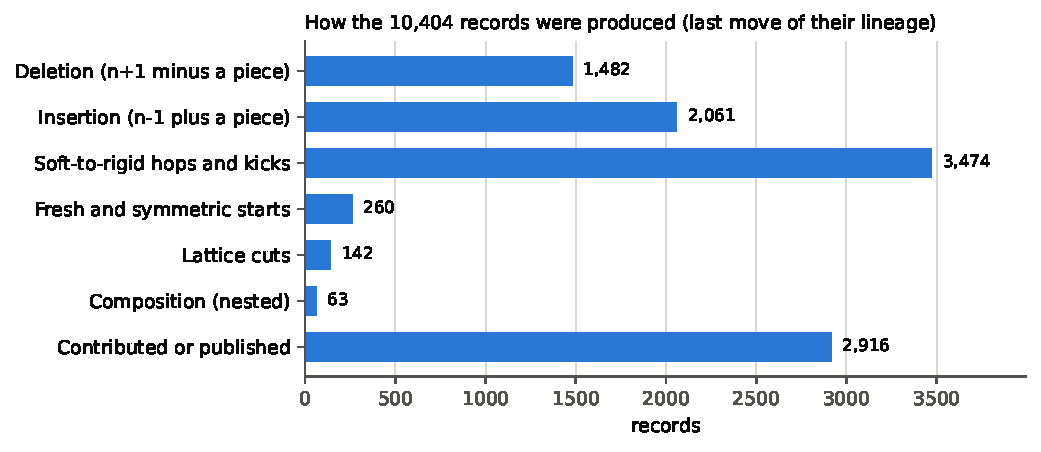
\includegraphics[width=0.86\textwidth]{fig_lineage.pdf}
\caption{The last move in each record's lineage. Deletion and insertion together produced a third of the catalogue.}
\label{fig:lineage}
\end{figure}

\begin{figure}[t]
\centering
\includegraphics[width=\textwidth]{fig_gallery.pdf}
\caption{Pattern classes in records. Top: an FCC shell, a Cartesian shell and the triakis recursion (all proved in Lean at the exact scale). Bottom: a two-orientation window (orientation classes in blue and orange), a cube tiling, and a proven-optimal $n=2$ record.}
\label{fig:gallery}
\end{figure}

\section{Formalization}\label{sec:formal}

All theorems cited above are in \code{lean-optimality/} (Lean 4.31, Mathlib). The continuous-integration audit checks that every one depends only on the axioms \texttt{propext}, \texttt{Classical.choice} and \texttt{Quot.sound}.

\begin{center}\footnotesize
\begin{tabularx}{\textwidth}{>{\raggedright}p{3.1cm} >{\raggedright}X >{\raggedright\arraybackslash}p{4.0cm}}
\toprule
Module & Theorems & Content \\
\midrule
\code{Basic.lean} & \code{Packing.restrict} & deletion \\
\code{Patterns.lean} & \code{Packing.mono}, \code{compose}, \code{selfCompose}, \code{pow} & scale monotonicity, composition \\
 & \code{of_separators}, \code{smulBoth} & separator certificates (F), rescaling \\
 & \code{voronoi_disjoint}, \code{voronoi_packing}, \code{lattice_window} & Voronoi windows \\
\code{Windows.lean} & \code{rdo_window}, \code{tcu_window}, \code{rdo19/44/93}, \code{tcu56} & exact FCC and cubic windows \\
\code{Triakis.lean} & \code{ktt4}, \code{triakis_recursion}, \code{ktt16}, \code{ktt64} & the recursion $4^k$ at $(5/3)^k$ \\
\code{Relations.lean} & \code{transfer_piece}, \code{transfer_container}, \code{optimal_plateau_of_*} & transfer; extremal bound plus deletion \\
\code{PrismCube.lean}, \code{TriPrism\-Cube.lean}, \code{PolyPrism.lean} & \code{width_le}, \code{centre_of_box}, \code{pcentre}, 13 records & widths and the box centre lemma; optimal prisms in a cube \\
\code{LemmaF5.lean}, \code{LemmaF5\-Sphere.lean}, \code{Penteracts.lean} & \code{lemmaF5}, \code{band5}, \code{centre5}, \code{hc5inhc5_plateau} & the cube centre lemma in 5D; 30 records \\
\bottomrule
\end{tabularx}
\end{center}

The formal results are of three kinds. The mechanisms and the relations between them are proved for arbitrary bodies and containers: deletion, monotonicity, composition, transfer, separator certificates, Voronoi windows and the passage from an extremal bound to an optimal plateau. The optimality results are lower bounds matched by exact constructions (Section~\ref{sec:extremal}). The exact instances are specific packings at exact algebraic scales; the catalogue certifies their padded counterparts by exact arithmetic. Descriptive classes (layers, orientation classes, symmetry) are measurements, not theorems.

\section{Limitations}\label{sec:limits}

The classification is empirical: a record can belong to several classes, and the thresholds (tolerances, the cap of four orientation classes for windows, the gap $N-k\le6$ for inheritance) are choices. On square antiprisms the arrows reproduce values PingYou Ltd announced first and produced no bound below theirs; their submitted witnesses are now the records. Contact graphs depend on the $10^{-5}$ threshold. The one-piece scales behind the transfer bounds are numerical, so the transfer comparison is a measurement, although each transfer construction, once made explicit, is certified like any other record. Closed forms are conjectures until their contact systems are solved exactly. The formal layer proves the mechanisms and the listed instances, not the optimality of the windows. Only the \nProven{} records counted in Section~\ref{sec:extremal} are proven optimal.

\section*{Acknowledgements}
The arrows of Section~\ref{sec:arrows}, their F and P steps, and many of the number patterns of Sections~\ref{sec:compose}--\ref{sec:windows} are due to PingYou Ltd~\cite{pingSixteen,pingArrows}. Their constructions also include the corner completion, golden shells and layers, finite Welsh windows, FCC shells and windows, the Cartesian shell, and mixed, quadratic-field and column layers. The catalogue combines searches and contributions by PingYou Ltd, \code{konoha-ily2} (Hirotaka Nakano), PolyPack (Michael Sinko), Berthold, Kamp, Mexi, Pokutta and P\'olik~\cite{berthold2026}, Hiroaki Hosono~\cite{hosono}, Stian, Ryan Xu and others. Soft-to-rigid continuation is due to Yohei Nakajima~\cite{nakajima2026}. AI coding and drafting tools, including Claude (Anthropic), assisted implementation, analysis, formalization and manuscript preparation under human direction. The Lean build and the exact certificates, not the tools, are the evidence for the formal and certified claims.

\begin{thebibliography}{99}
\bibitem{archive} A. Zarzuelo Urdiales and contributors. \emph{Polyhedra in Polyhedra: certified finite packings}. \url{https://github.com/alejandrozu/platonic-packing}, \url{https://polyhedrainpolyhedra.wiki}, 2026.
\bibitem{zarzueloMethods} A. Zarzuelo Urdiales. \emph{Certified finite packings of Platonic solids: a generalized soft-to-rigid search and its computational development}. 2026. \url{https://doi.org/10.5281/zenodo.23306098}.
\bibitem{zarzueloPatterns} A. Zarzuelo Urdiales. \emph{Finite polyhedral fits: discrete scale jumps, orientational domains, and contact structure in 351 certified constructions}. 2026. \url{https://doi.org/10.5281/zenodo.23306126}.
\bibitem{nakajima2026} Y. Nakajima. \emph{Soft-to-Rigid: Shape Continuation as an Alternative Search for Packing Congruent Shapes}. arXiv:2610.14463v1, 2026. \url{https://arxiv.org/abs/2610.14463}.
\bibitem{berthold2026} T. Berthold, D. Kamp, G. Mexi, S. Pokutta and I. P\'olik. \emph{Out-of-the-Box Global Optimization for Packing Problems: New Models and Improved Solutions}. arXiv:2605.04850, 2026.
\bibitem{hosono} H. Hosono. \emph{square-packing}: computer-assisted optimality proofs for cube packings. \url{https://github.com/wand125/square-packing}, 2026.
\bibitem{pingSixteen} PingYou Ltd. \emph{Sixteen constructions, exact structure} (illustrated notes on number patterns in the catalogue), 5 November 2026.
\bibitem{pingArrows} PingYou Ltd. \emph{Published packings vs.\ strongest verified constructions: square antiprisms, $N=1$--20}, and \emph{The four arrows, specified as numerical procedures}, 6 November 2026.
\bibitem{ping79} PingYou Ltd. Whole-body polytope inclusion construction, contribution \#79, 2026. \url{https://github.com/alejandrozu/platonic-packing/issues/79}.
\bibitem{mathlib} The mathlib Community. The Lean mathematical library. In \emph{CPP 2020}, 367--381.
\bibitem{conwaySloane} J. H. Conway and N. J. A. Sloane. \emph{Sphere Packings, Lattices and Groups}, 3rd ed. Springer, 1999.
\end{thebibliography}

\end{document}
